Two listening experiments were conducted in an acoustically-treated listening room,
where the listener was seated and given a pair of headphones.
Four subjects, all male, ages 25--30 years, participated in the experiments;
each subject is an experienced audio engineer or researcher.
Prior to the experiments, each subject's HRTFs were measured in an anechoic chamber.
These HRTFs were measured also as part of an ongoing project to compile a database of measured HRTFs \citep{Sridhar2017}.
The procedures employed to collect and process these measurements are reproduced in \apxref{chap:A4_HRTF_Measurements}.

Each subject's HRTFs were used to generate an individualized ambisonics-to-binaural rendering configuration for the ambiX binaural decoder plug-in \citep{Kronlachner2013,ambiXPlugInURL}.
In this decoder, we performed a basic (pseudoinverse) ambisonic decoding (see \eqnref{eq:02_Acoustical_Theory:PinvDecoder}) for a 36-node Fliege grid and filtered each virtual loudspeaker's signal by the nearest measured HRTF.
This decoder was generated using an early version of the SOFA/ambiX binaural rendering (SABRE) toolkit, which was developed by the present author and is described in \apxref{chap:A2_SABRE_Toolkit}.
The headphones (Stax SR-009) were equalized for each subject using a regularized, least-squares equalization filter \citep{ScharerLindau2009}.

The test samples were produced using the weighted average method and a regularized least-squares interpolation method (described in \secreftwo{sec:03_Navigation_Techniques:XF_Technique}{sec:08_Proposed_Method:Reg-LS_Technique}, respectively), employed for microphone spacings of 10, 30, or 50~cm.
The test samples were rendered from 4\textsuperscript{th}-order ambisonics room impulse responses for microphone positions distributed on both sides of the listening position, as illustrated by the empty circles in \figref{fig:Test_Geometry}.
For the localization test, these impulse responses were measured with a 32-capsule spherical microphone array, using phase-controlled exponential sine sweeps and an exact deconvolution of the recorded signals by the input signal, as described in \apxref{chap:A5_Impulse_Response}.
For the coloration test, on the other hand, the impulse responses were simulated using a MATLAB-based room acoustics simulator%
\footnote{In this work, we used the Multichannel Room Acoustics Simulator (\textsc{MCRoomSim}) package \citep{Wabnitz2010,MCRoomSimURL}.}
with a room model similar in size and acoustics to the actual listening room.
Also included in each test were reference samples, measured at the listening position and for which no interpolation was performed.
All stimuli were presented at levels between 60~dB and 78~dB (A-weighted), $\pm4$~dB.

% Diagram of source/mic positions
\begin{figure}[t]
\centering
  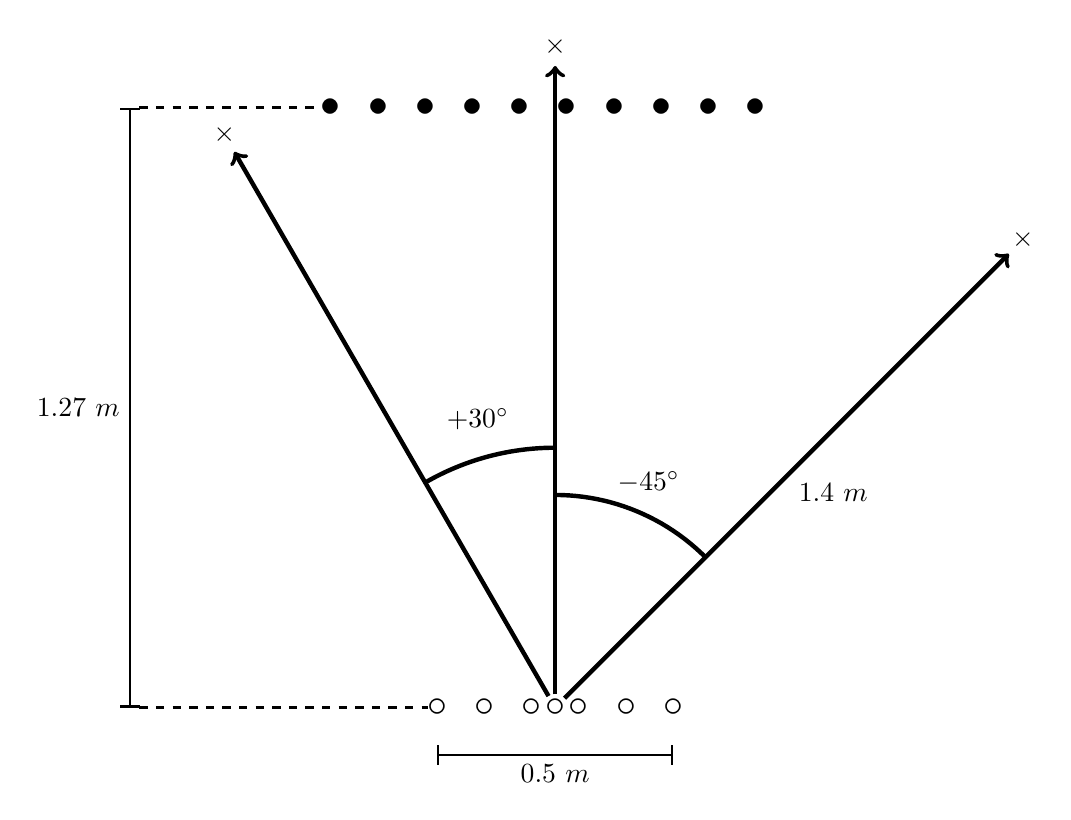
\begin{tikzpicture}[scale=6]
% Parameters
\def\radius{1.4};
\def\arrowStart{0.02};
\def\arrowScale{0.97};
\def\arcRadius{0.5};
\def\micSpacing{0.1};
\def\spkrSpacing{0.05};
\def\spkrDistance{1.27};
\def\offset{0.02};
\pgfmathsetmacro\colLefty{cos(-30)*\radius}
\pgfmathsetmacro\colLeftx{sin(-30)*\radius}
\pgfmathsetmacro\colCentery{cos(0)*\radius}
\pgfmathsetmacro\colCenterx{sin(0)*\radius}
\pgfmathsetmacro\colRighty{cos(45)*\radius}
\pgfmathsetmacro\colRightx{sin(45)*\radius}
\pgfmathsetmacro\arcLefty{cos(-15)*1.1*\arcRadius}
\pgfmathsetmacro\arcLeftx{sin(-15)*1.1*\arcRadius}
\pgfmathsetmacro\arcRighty{cos(22.5)*0.9*\arcRadius}
\pgfmathsetmacro\arcRightx{sin(22.5)*0.9*\arcRadius}

% Arrows
\draw[ultra thick,->] ({\arrowStart*\colLeftx},{\arrowStart*\colLefty}) -- (\arrowScale*\colLeftx,\arrowScale*\colLefty);
\draw[ultra thick,->] ({\arrowStart*\colCenterx},{\arrowStart*\colCentery}) -- (\arrowScale*\colCenterx,\arrowScale*\colCentery);
\draw[ultra thick,->] ({\arrowStart*\colRightx},{\arrowStart*\colRighty}) -- (\arrowScale*\colRightx,\arrowScale*\colRighty);
\node[below right] at (0.5*\colRightx,0.5*\colRighty){$1.4~\text{m}$};
\node at (\colLeftx,\colLefty){$\times$};
\node at (\colCenterx,\colCentery){$\times$};
\node at (\colRightx,\colRighty){$\times$};

% Distances
\draw[thick,|-|] (-2.5*\micSpacing,-0.1) -- (2.5*\micSpacing,-0.1) node[below, pos=0.5]{$0.5~\text{m}$};
\draw[thick,|-|] (-0.9,0) -- (-0.9,\spkrDistance) node[left, pos=0.5]{$1.27~\text{m}$};
\draw[thick, dashed] (-0.9+\offset,\spkrDistance) -- (-9.5*\spkrSpacing-\offset,\spkrDistance);
\draw[thick, dashed] (-0.9+\offset,0) -- (-2.5*\micSpacing-\offset,0);

% Arcs
\draw[ultra thick,domain=45:90] plot ({0.9*\arcRadius*cos(\x)}, {0.9*\arcRadius*sin(\x)});
\draw[ultra thick,domain=90:120] plot ({1.1*\arcRadius*cos(\x)}, {1.1*\arcRadius*sin(\x)});
\node at (1.15*\arcLeftx,1.15*\arcLefty){$+30^\circ$};
\node at (1.15*\arcRightx,1.15*\arcRighty){$-45^\circ$};

% Mic positions
\node at (-2.5*\micSpacing,0){\Large $\circ$};
\node at (-1.5*\micSpacing,0){\Large $\circ$};
\node at (-0.5*\micSpacing,0){\Large $\circ$};
\node at (0*\micSpacing,0){\Large $\circ$};
\node at (0.5*\micSpacing,0){\Large $\circ$};
\node at (1.5*\micSpacing,0){\Large $\circ$};
\node at (2.5*\micSpacing,0){\Large $\circ$};

% Speaker positions
\node at (-9.5*\spkrSpacing,\spkrDistance){\Large $\bullet$};
\node at (-7.5*\spkrSpacing,\spkrDistance){\Large $\bullet$};
\node at (-5.5*\spkrSpacing,\spkrDistance){\Large $\bullet$};
\node at (-3.5*\spkrSpacing,\spkrDistance){\Large $\bullet$};
\node at (-1.5*\spkrSpacing,\spkrDistance){\Large $\bullet$};
\node at (0.5*\spkrSpacing,\spkrDistance){\Large $\bullet$};
\node at (2.5*\spkrSpacing,\spkrDistance){\Large $\bullet$};
\node at (4.5*\spkrSpacing,\spkrDistance){\Large $\bullet$};
\node at (6.5*\spkrSpacing,\spkrDistance){\Large $\bullet$};
\node at (8.5*\spkrSpacing,\spkrDistance){\Large $\bullet$};
\end{tikzpicture}
  \caption[Diagram of microphone and source positions used in the listening tests.]{
  Diagram of microphone and source positions used in the listening tests.
  The empty circles indicate the microphone positions,
  the filled circles indicate the source positions used in the localization test, and
  the crosses indicate the source positions used in the coloration test.}
  \label{fig:Test_Geometry}
\end{figure}

\subsection{Localization test}\label{sec:05_Proposed_Models:Localization_Test}
To measure perceived source localization, we conducted a virtual source localization test, in which the listener was seated approximately $1.27$~m in front of a horizontal linear array of 30 transducers spaced 5~cm apart (note that the array served only as a visual reference to promote an externalized perception of the sound by the listener).
An infrared head-tracking device (NaturalPoint TrackIR) was used to maintain a stationary sound field as the subject's head rotated.
The test consisted of 1 training round followed by 5 rounds of testing, with optional short breaks in between each round for the subject to stand up and take off the headphones.
In each round, the subject was presented with 14 randomly-selected samples (2 references and 12 test samples in each round), all of which were a short ($\sim2$~second) clip of male English speech.
The graphical user interface (GUI) presented to the subject is shown in \figref{fig:05_Proposed_Models:Localization_GUI} and the sheet of instructions provided to the subject is shown in \figref{fig:05_Proposed_Models:Localization_Instructions} (at the end of this chapter).
The intended source directions produced in the test corresponded to 10 of the 30 transducers, spanning approximately $\pm20^\circ$ azimuth on the horizontal plane, as illustrated by the filled circles in \figref{fig:Test_Geometry}.
The subject was asked to identify the direction from which the sound appeared to originate, and subsequently face it.
The subject's head-angle (obtained from the head-tracking device) was then captured and recorded as the perceived direction of the source.
The subject was able to repeat each sample any number of times until confident about the location of the source.

\begin{figure}[t]
  \centering
  \setlength{\fboxsep}{0pt}
  \setlength{\fboxrule}{1pt}
  \fbox{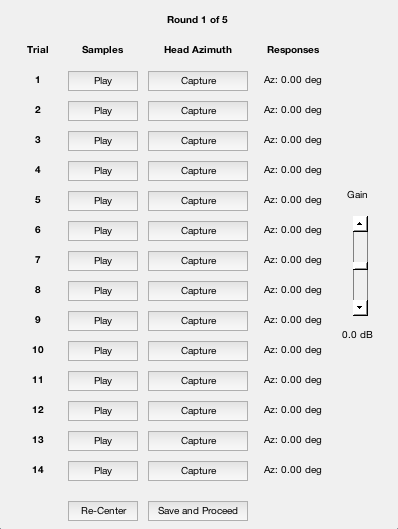
\includegraphics[width=0.58\textwidth]{05_proposed_models/figures/LocalizationTestGUI}}
  \caption{Screenshot of the GUI for the localization test.}
  \label{fig:05_Proposed_Models:Localization_GUI}
\end{figure}

\subsection{Coloration test}\label{sec:05_Proposed_Models:Coloration_Test}
To collect subjective ratings of coloration, we conducted an \citet{ITU-R-BS.1534-3} MUSHRA (MUltiple Stimuli with Hidden Reference and Anchor) test,
administered in the same listening room and with the same headphones, but without head-tracking.%
\footnote{The loudspeaker array which served as a visual reference for the localization test was still present for this test, but the subjects were informed that it no longer corresponded to the signals they would be hearing.}
The test consisted of 1 training round followed by 3 rounds of testing, with optional short breaks between rounds.
In each round, the subject was presented with 9 ``test samples'' (actually 6 test samples, 2 anchors, and a hidden reference) and a labeled reference sample, all of which were a short ($\sim3$~second) clip of pink noise.
The GUI presented to the subject is shown in \figref{fig:05_Proposed_Models:Coloration_GUI} and the sheet of instructions provided to the subject is shown in \figref{fig:05_Proposed_Models:Coloration_Instructions} (at the end of this chapter).
The so-called ``low anchor'' used was the standard $3.5$~kHz low-pass-filtered version of the reference \citep{ITU-R-BS.1534-3}; the second anchor used was a high-shelf-filtered version of the reference, with $+6$~dB of gain applied above $7$~kHz.
The samples were randomly-ordered, but all samples in each round were from a single intended source direction.
The intended source directions produced in the test corresponded to $-45^\circ,~0^\circ,~30^\circ$ azimuth on the horizontal plane, as illustrated by the crosses in \figref{fig:Test_Geometry}.
The subject was asked to judge (and rate on a scale from 0--100) the extent to which each test sample \textit{differs}, in terms of the tonal coloration only, from the labeled reference sample.
As is standard in a MUSHRA test, a rating of 100 indicates that the sample is \textit{indistinguishable} from the reference,
while any rating less than 100 indicates that the sample differs from the reference.
All responses for each round and each subject were linearly mapped (if necessary) such that the low anchor obtained a rating of 0.
In the present dataset, all subjects correctly identified the hidden reference and rated it 100.
The subject was able to repeat each sample (and the labeled reference) any number of times until satisfied with the ratings for that round.

\begin{figure}[t]
  \centering
  \setlength{\fboxsep}{0pt}
  \setlength{\fboxrule}{1pt}
  \fbox{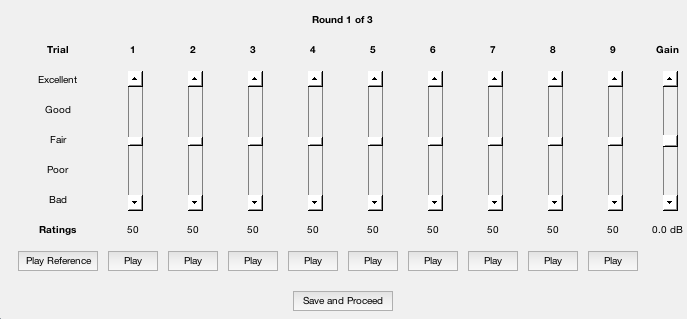
\includegraphics[width=0.99\textwidth]{05_proposed_models/figures/ColorationTestGUI}}
  \caption{Screenshot of the GUI for the coloration test.}
  \label{fig:05_Proposed_Models:Coloration_GUI}
\end{figure}